\chapter{Projet Bac à Sable} % Main chapter title

\section{Introduction}

Mon premier projet chez WeVii est le projet bac à sable.
Il m’a permis de faire mes premiers pas dans le monde du DevOps.

\section{Technologies utilisées}

Les principales technologies utilisées dans ce projet sont :
\begin{multicols}{2}
    \begin{itemize}
        \item JavaScript : Un langage de programmation utilisé pour le web.
        \item Angular : Un outil qui aide à créer des applications web.
        \item Node.js : Un environnement pour exécuter du code JavaScript sur un serveur.
        \item Docker : Un outil qui permet de mettre une application dans un "conteneur" pour qu'elle puisse fonctionner n'importe où.
        \item Kubernetes : Un système pour gérer et orchestrer les conteneurs Docker.
        \item Helm : Un outil pour gérer des applications Kubernetes.
        \item Serveur Cloud : Un ordinateur qui exécute des applications sur Internet.
        \item ArgoCD : Un outil pour automatiser le déploiement d'applications.
        \item GitHub : Un site web pour stocker et partager du code.
        \item GitHub Actions : Un outil pour automatiser des tâches comme le déploiement.
        \item MongoDB : Une base de données pour stocker des informations.
    \end{itemize}
\end{multicols}

\section{Objectif du projet}

L’objectif de ce projet était de faire une petite application qui affichait « Hello » et un prénom ajouté par l’utilisateur, l’application affiche « World » par défaut.

\begin{figure}[ht]
    \centering
    \begin{minipage}{.45\textwidth}
        \centering
        
\includegraphics[width=\linewidth]{image/sbHelloWorld}
        \caption{Application lors de la première connexion}
        \label{fig:sbHelloWorld}
    \end{minipage}%
    \hfill
    \begin{minipage}{.45\textwidth}
        \centering
        
\includegraphics[width=\linewidth]{image/sbHelloPaul}
        \caption{Une fois un prénom ajouté}
        \label{fig:sbHelloPaul}
    \end{minipage}
\end{figure}

L’application devait se souvenir du prénom grâce aux cookies (des petits fichiers stockés sur l'ordinateur de l'utilisateur) et donc l’enregistrer.

\begin{figure}[ht]
    \centering
    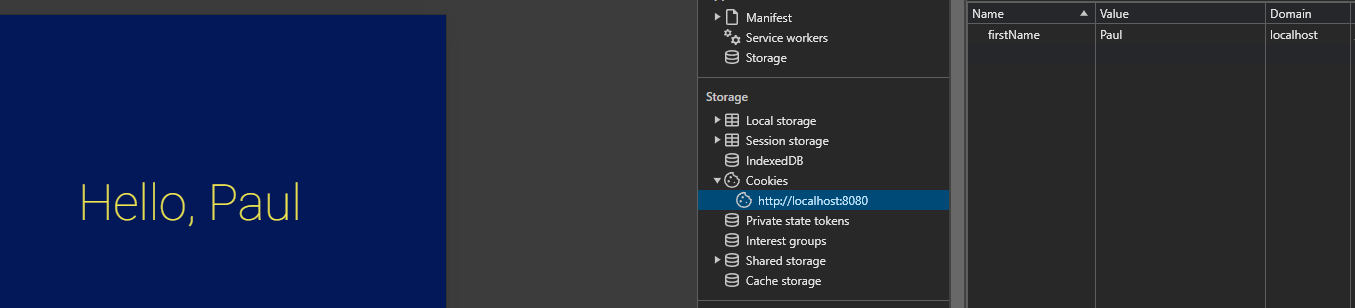
\includegraphics[width=0.7\textwidth]{image/sbCookie}
    \caption{Cookie stocké sur l'ordinateur de l'utilisateur}
    \label{fig:sbCookie}
\end{figure}

Elle a dû être hébergée sur un serveur Web, ce qui a permis de découvrir la conteneurisation (mettre l'application dans un conteneur), l’orchestration (gérer plusieurs conteneurs) ainsi que le déploiement continu (mettre à jour l'application automatiquement).

Pour empêcher que l'application soit victime de cyber-attaques, nous avons appliqué de bonnes pratiques de sécurité, comme cacher les clés API et les URLs sensibles en utilisant des variables d'environnement ou des secrets.

\section{Conception}

\subsection{Formation et apprentissage}

Dans un premier temps, afin de réaliser ce projet, l’essentiel était de se former sur JavaScript.
De plus, étant donné qu’à l’IUT nous faisions du JavaScript, cela m’a permis de progresser plus rapidement.
En parallèle, j’ai dû comprendre et apprendre le fonctionnement du Framework Angular et comment créer une API CRUD (une interface qui permet de créer, lire, mettre à jour et supprimer des données dans une base de données).

\subsection{Développement}

Une fois les connaissances acquises, j’ai pu commencer à développer l’application. L’application est divisée en deux parties :

\begin{itemize}
    \item \textbf{FrontEnd} : La partie visible de l’application, réalisée avec Angular.
    \begin{figure}[H]
        \centering
        \begin{minipage}{.6\textwidth}
            \centering
            \begin{lstlisting}[language=Java]
getFirstName(): Observable<{ string }> {
    const firstName = this.cookieService.get('firstName');
    return this.http.get<{ firstName: string }>(
      `${this.apiUrl}/firstName?cookie=${firstName}`
    );
}
            \end{lstlisting}
            \caption{Exemple de code du FrontEnd : Récupération du prénom via un service de cookies et une requête HTTP GET.}
        \end{minipage}
    \end{figure}

    \item \textbf{BackEnd} : La partie qui fonctionne côté serveur, réalisée avec Node.js.
    \begin{figure}[H]
        \centering
        \begin{minipage}{.6\textwidth}
            \centering
            \begin{lstlisting}[language=Java]
app.get('/backend/firstName', async (req, res) => {
  const userId = req.query.userId;
  console.log("ID de l'utilisateur dans la requête :", userId);
  if (!userId) {
    res.json({
    'World'
});
    return;
  }
  try {
    const user = await User.findById(userId);
    console.log('Utilisateur récupéré depuis MongoDB :', user);
    if (!user) {
      res.json({ firstName: 'World' });
      return;
    }
    res.json({ firstName: user.firstName });
  } catch (error) {
    console.error('Erreur lors de la récupération du prénom depuis MongoDB :', error);
    res.status(500).json({ error: 'Erreur lors de la récupération du prénom.' });
  }
});
            \end{lstlisting}
            \caption{Exemple de code du BackEnd : Récupération du prénom de l'utilisateur depuis la base de données.}
        \end{minipage}
    \end{figure}
\end{itemize}

Le développement a pris du temps, avec des erreurs et des retours en arrière fréquents, mais cela m'a beaucoup motivé et m'a donné envie de progresser.
Une fois le développement terminé, nous avons acquis de nombreuses compétences et nous étions prêts pour le déploiement.

\section{Déploiement}

Le déploiement consiste à mettre l’application en ligne sur un serveur.
Le chercheur m’a fourni un serveur cloud sécurisé par une connexion SSH. Il m’a donné des instructions afin de me former, et m'a recommandé de conteneuriser l’application sous forme de conteneur Docker.

\begin{figure}[H]
    \centering
    \begin{minipage}{.8\textwidth}
        \centering
        \begin{lstlisting}[language=Go]
 FROM node:18.18.0
 WORKDIR /app
 COPY package*.json ./
 RUN npm install -g npm@10.2.1
 RUN npm install
 RUN npm audit fix
 EXPOSE 3000
 COPY app.js .
 COPY config.json .
 CMD ["node", "app.js"]
        \end{lstlisting}
        \caption{Exemple de code d'un fichier Docker pour conteneuriser le backend.}
    \end{minipage}
\end{figure}

Les conteneurs sont légers et faciles à transporter, ce qui optimise l’espace et permet de faire fonctionner l’application directement sur le serveur. Le chercheur s’est occupé de la partie infrastructure, en mettant en place un DNS pour vérifier si l’application fonctionnait. Après avoir réalisé la première partie du déploiement et appliqué les bonnes pratiques de cybersécurité, nous avons pu ajouter des fonctionnalités supplémentaires pour augmenter la difficulté et améliorer l’application.

\section{Amélioration de l’application}

Le chercheur m'a fait découvrir Kubernetes, une technologie très utilisée pour le déploiement et l'orchestration de conteneurs. Kubernetes permet d'orchestrer des conteneurs, gérer leur cycle de vie, et assurer le bon fonctionnement de l'application grâce à des outils de déploiement continu. En utilisant Kubernetes, j'ai pu mettre en place un déploiement continu de manière simple et efficace pour automatiser au mieux les tâches répétitives.

\section{Conclusion}

Une fois le déploiement finalisé et fonctionnel, le chercheur a jugé que nous pouvions partir sur un projet plus concret et complet. Ce projet était très pédagogique mais peu concret d’un point de vue professionnel. Il m’a permis de découvrir comment réaliser un projet et quelles sont les étapes pour y arriver. De plus, il m’a poussé à me renseigner sur toutes les technologies que j’ai été amené à utiliser. Ce projet a été un très bon point de départ car il n’a pas été complexe dans sa forme mais il permet de pratiquer de nombreux domaines de compétences dans le DevOps. J’ai apprécié réaliser ce projet, et malgré les difficultés rencontrées, je reste passionné.
